\documentclass[10pt,a4paper]{article}
\usepackage[utf8]{inputenc}

% Define the page margin
\usepackage[margin=3cm]{geometry}

% Better typography (font rendering)
\usepackage{microtype}

% Math environments and macros
\usepackage{amsmath}
\usepackage{amsfonts}
\usepackage{amssymb}
\usepackage{amsthm}

% Define \includegraphics to include graphics
\usepackage{graphicx}

% Draw graphics from a text description
\usepackage{tikz}

% Syntax highlighting
\usepackage{minted}

% Set global minted options
\setminted{linenos, autogobble, frame=lines, framesep=2mm}

% Import the comment environment for orgtbl-mode
\usepackage{comment}

% Do not indent paragraphs
\usepackage{parskip}

\title{Databases, Sheet 11}
\author{Marten Lienen (03670270)}

\begin{document}

\maketitle

\section*{Exercise 1}

Da auf jeder Seite ca. 100 Einträge stehen, muss es insgesamt ungefähr $\frac{10^{10}}{10^{2}} = 10^{8}$ Seiten geben.
Das Verzeichnis kann nur in 2er-Potenzen wachsen, weshalb dessen Größe die nächsthöhere 2er-Potenz sein muss.
\begin{equation*}
  \log_{2}(10^{8}) = 8 \cdot \log_{2}(10) \approx 26.6
\end{equation*}
Das Verzeichnis hat also $2^{27}$ Einträge, was bei einem Speicherplatzverbrauch von $4$ Byte pro Verweis eine Größe von $2^{27} \cdot 4 = 2^{29} = 536870912$ Byte bzw. $539$ GB ergibt.

\section*{Exercise 2}

\subsection*{Part 1)}

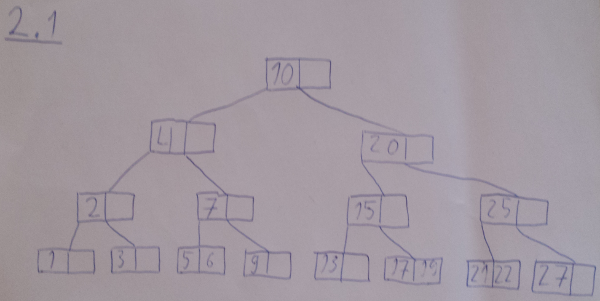
\includegraphics[width=\textwidth]{sheet-11/exercise-2-1}

\subsection*{Part 2)}

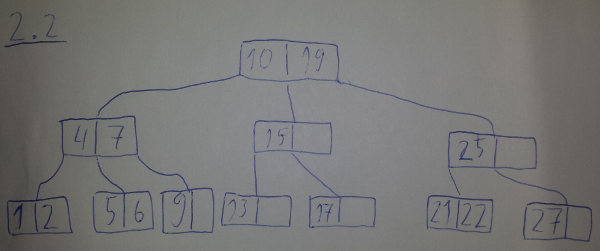
\includegraphics[width=\textwidth]{sheet-11/exercise-2-2}

\section*{Exercise 3}

Die Speicherauslastung ist sehr schlecht, weil durch das Einfügen in aufsteigender Reihenfolge der Baum immer nur nach rechts geteilt wurde.
Ein Einfügen in zufälliger Reihenfolge könnte diese Problem mit hoher Wahrscheinlichkeit umgehen.

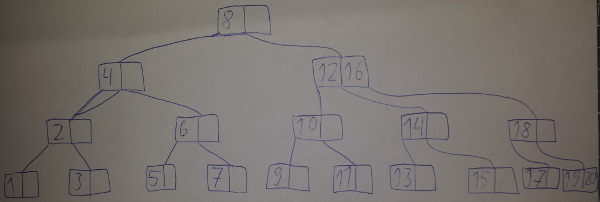
\includegraphics[width=\textwidth]{sheet-11/exercise-3}

\section*{Exercise 4}

Die zwei schweren Stellen sind das Aufteilen von Knoten und in welchen Teilbaum ein neuer Knoten eingefügt werden soll, weil nicht wirklich definiert ist, nach welchen Kriterien vorgegangen werden soll.
Ich bin nun so vorgegangen, dass sich die zusammengefassten Knoten möglichst wenig unterscheiden bzw. der eingefügte Knoten von dem ausgewählten Teilbaum.
Zur Abstandsbestimmung habe ich erst das Alter betrachtet und bei Gleichstand auf das Gehalt zurückgegriffen und so weiter.

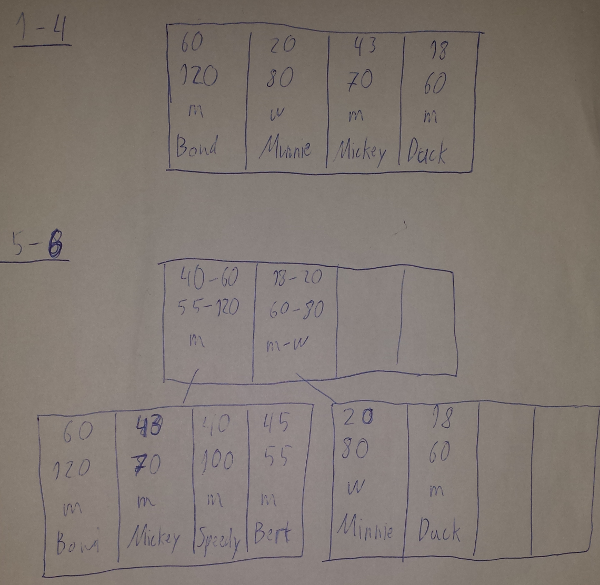
\includegraphics[width=\textwidth]{sheet-11/exercise-4}

\section*{Exercise 5}

$BCF$ ist ein Kandidatenschlüssel, weil von ihm die gesamte Relation funktional abhängt und er nicht minimiert werden kann.
Ein weiterer Kandidat wäre $CDF$.
$C$ und $F$ müssen immer dabei sein, weil sie von nichts funktional abhängen.
$A$ und $E$ sind nie drin, weil sie von $C$ abhängen, was immer dabei ist.
Schlussendlich braucht man $D$ nicht, wenn man $B$ hat, und andersherum, sodass dies die einzigen Kandidaten sind.

Man erhält die zwei Relationenschemata $BDA$ und $BCEF$, wobei die Schlüssel $B$ und $BCEF$ sind.
Es gibt keine weiteren Schemata, weil sich keine der funktionalen Abhängigkeiten auf $BCEF$ übertragen lassen und somit $BCEF$ der einzige Superschlüssel in $BCEF$ ist.

Wenn man die kanonische Überdeckung dieser FDs bildet, erhält man noch weitere.
Diese sind für den Dekompositionsalgorithmus jedoch nicht wichtig, weil er keine Abhängigkeitserhaltung garantiert.
Es reicht deshalb mit einer minimalen beschreibenden Menge von FDs zu arbeiten.

\end{document}
